
\documentclass[a4paper,12pt]{scrbook}
\usepackage{amsmath,amssymb,amsthm}
\usepackage{fancyvrb}
\usepackage{parskip}
\usepackage{lastpage}
\usepackage{verbatim,boxedminipage,enumitem}
\usepackage{ifthen}
\usepackage{color,graphicx}
\usepackage{pgf}
\usepackage{longtable}
\usepackage{upquote}
%\usepackage[all]{xy}
\usepackage{tobiShell}
\usepackage{tikz}
\usetikzlibrary{automata}
\usetikzlibrary{arrows}
\usepackage{pgf,pgfarrows,pgfnodes}
\usepackage{pgfplots}
\usepackage{circuitikz}
\usetikzlibrary{circuits}
\usetikzlibrary{circuits.logic.US}
\usepackage{mymath}
\usepackage{python}
%------------------------------------------------------------------
% Verbatim for console window - single line frame, no line numbers
%------------------------------------------------------------------
\DefineVerbatimEnvironment%
 {console}{Verbatim}
 {frame=single}

%--------------------------------------------------------
% Remove the vertical spacing before and after Verbatim.
%--------------------------------------------------------
\usepackage{atbeginend}
\BeforeBegin{console}{\mbox{}\\ \begin{minipage}{\textwidth}\vspace{3pt}}
\AfterEnd{console}{\vspace{4pt} \end{minipage} \\ }

\begin{document}
\thispagestyle{empty}

\begin{center}
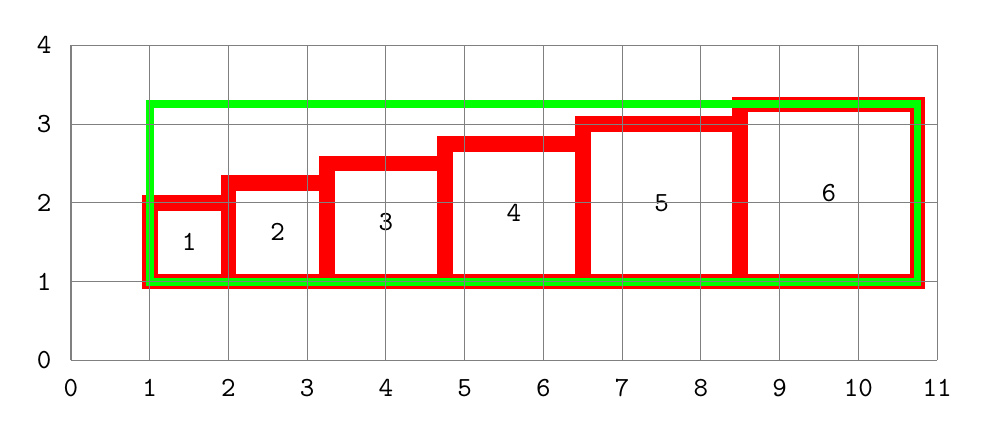
\begin{tikzpicture}

\draw (1.5, 1.5)
  node[draw, line width=0.2cm, , color=red,
       rounded corners=0cm, inner sep=0cm] {

\begin{minipage}[t][1.0cm]{1.0cm}
\mbox{}

\end{minipage}

};\draw (1.5, 1.5) node[color=black] {{\texttt{1}}};
\draw (2.625, 1.625)
  node[draw, line width=0.2cm, , color=red,
       rounded corners=0cm, inner sep=0cm] {

\begin{minipage}[t][1.25cm]{1.25cm}
\mbox{}

\end{minipage}

};\draw (2.625, 1.625) node[color=black] {{\texttt{2}}};
\draw (4.0, 1.75)
  node[draw, line width=0.2cm, , color=red,
       rounded corners=0cm, inner sep=0cm] {

\begin{minipage}[t][1.5cm]{1.5cm}
\mbox{}

\end{minipage}

};\draw (4.0, 1.75) node[color=black] {{\texttt{3}}};
\draw (5.625, 1.875)
  node[draw, line width=0.2cm, , color=red,
       rounded corners=0cm, inner sep=0cm] {

\begin{minipage}[t][1.75cm]{1.75cm}
\mbox{}

\end{minipage}

};\draw (5.625, 1.875) node[color=black] {{\texttt{4}}};
\draw (7.5, 2.0)
  node[draw, line width=0.2cm, , color=red,
       rounded corners=0cm, inner sep=0cm] {

\begin{minipage}[t][2.0cm]{2.0cm}
\mbox{}

\end{minipage}

};\draw (7.5, 2.0) node[color=black] {{\texttt{5}}};
\draw (9.625, 2.125)
  node[draw, line width=0.2cm, , color=red,
       rounded corners=0cm, inner sep=0cm] {

\begin{minipage}[t][2.25cm]{2.25cm}
\mbox{}

\end{minipage}

};\draw (9.625, 2.125) node[color=black] {{\texttt{6}}};
\draw (5.875, 2.125)
  node[draw, line width=0.1cm, , color=green,
       rounded corners=0cm, inner sep=0cm] {

\begin{minipage}[t][2.25cm]{9.75cm}
\mbox{}

\end{minipage}

};\draw[gray] (0.0,0.0) -- (0.0,4);
\draw[gray] (1.0,0.0) -- (1.0,4);
\draw[gray] (2.0,0.0) -- (2.0,4);
\draw[gray] (3.0,0.0) -- (3.0,4);
\draw[gray] (4.0,0.0) -- (4.0,4);
\draw[gray] (5.0,0.0) -- (5.0,4);
\draw[gray] (6.0,0.0) -- (6.0,4);
\draw[gray] (7.0,0.0) -- (7.0,4);
\draw[gray] (8.0,0.0) -- (8.0,4);
\draw[gray] (9.0,0.0) -- (9.0,4);
\draw[gray] (10.0,0.0) -- (10.0,4);
\draw[gray] (11.0,0.0) -- (11.0,4);
\draw[gray] (0.0,0.0) -- (11,0.0);
\draw[gray] (0.0,1.0) -- (11,1.0);
\draw[gray] (0.0,2.0) -- (11,2.0);
\draw[gray] (0.0,3.0) -- (11,3.0);
\draw[gray] (0.0,4.0) -- (11,4.0);
\draw(0, 0) node [font=\ttfamily, label=below:{\texttt{0}}] {};
\draw(1, 0) node [font=\ttfamily, label=below:{\texttt{1}}] {};
\draw(2, 0) node [font=\ttfamily, label=below:{\texttt{2}}] {};
\draw(3, 0) node [font=\ttfamily, label=below:{\texttt{3}}] {};
\draw(4, 0) node [font=\ttfamily, label=below:{\texttt{4}}] {};
\draw(5, 0) node [font=\ttfamily, label=below:{\texttt{5}}] {};
\draw(6, 0) node [font=\ttfamily, label=below:{\texttt{6}}] {};
\draw(7, 0) node [font=\ttfamily, label=below:{\texttt{7}}] {};
\draw(8, 0) node [font=\ttfamily, label=below:{\texttt{8}}] {};
\draw(9, 0) node [font=\ttfamily, label=below:{\texttt{9}}] {};
\draw(10, 0) node [font=\ttfamily, label=below:{\texttt{10}}] {};
\draw(11, 0) node [font=\ttfamily, label=below:{\texttt{11}}] {};
\draw(0, 0) node [font=\ttfamily, label=left:{\texttt{0}}] {};
\draw(0, 1) node [font=\ttfamily, label=left:{\texttt{1}}] {};
\draw(0, 2) node [font=\ttfamily, label=left:{\texttt{2}}] {};
\draw(0, 3) node [font=\ttfamily, label=left:{\texttt{3}}] {};
\draw(0, 4) node [font=\ttfamily, label=left:{\texttt{4}}] {};
\end{tikzpicture}

\end{center}

\end{document}
